%% LyX 2.2.1 created this file.  For more info, see http://www.lyx.org/.
%% Do not edit unless you really know what you are doing.
\documentclass[english]{article}
\usepackage[T1]{fontenc}
\usepackage[latin9]{inputenc}
\usepackage{geometry}
\geometry{verbose,tmargin=2.54cm,bmargin=2.54cm,lmargin=2.37cm,rmargin=3.17cm}
\usepackage{amsmath}
\usepackage{stackrel}
\usepackage{graphicx}
\usepackage{setspace}
\onehalfspacing

\makeatletter

%%%%%%%%%%%%%%%%%%%%%%%%%%%%%% LyX specific LaTeX commands.
%% Because html converters don't know tabularnewline
\providecommand{\tabularnewline}{\\}

\makeatother

\usepackage{babel}
\begin{document}

\title{Prediction of Stock Market with Sentiment Analysis}

\author{Lin Zeng(lz447), Qin Lu(ql224), Sizhang Zhao(sz459)}
\maketitle

\section{Idea}
\begin{quotation}
Stock market prediction is the core research area in trading and investment.
Stock price is determined by the behavior of human investors, and
the investers determine stock prices by using publicly available information
to predict the market future trend. Financial news can thus play a
significant role in influencing the stock trend as human react to
the information. Previous reasearch have suggested that there is some
lag between the time news article was released and the time the market
absorbed and reflected these information. So our main goal here is
to classify the news as our sentiment factor and use the sentiment
factor to determine the impact of the news on the stock price. 

In the first part of our research, we focus on sentiment analysis
with Google news in the whole finance division, and build up classification
models to measure the relationship between news sentiment and stock
index trend over time. Second, we add the sentiment factor to classify
the single stock up and down performances in SVM and neural network
models. Finally, we try to design a tradable portfolio based on our
sentiment factor and test its application in investments. 
\end{quotation}

\section{Data Scraping}
\begin{quotation}
Headers of financial news usually contain the impact of a certain
event to the whole market. For example, \emph{warn, volatility, decline,
plunge} are common phrases that are conceived as negative news to
market, and \emph{hike, allow, optimism, gain} are phrases that are
considered as positive ones. So in order to capture as much sentiment
information as possible for news each day, we use the headers of financial
news as our data set instead of the whole article.

We designe a web scraper to scratch the Google news headers in finance
division from January - October 2008 in daily basis. 

By locating the headers in source code from Google news, we use \emph{BeautifulSoup}
package in Python to scratch the headers in the search page by changing
the time zone in advanced search. We store news headers scratched
from Google news each day in separate \emph{.txt} file as the raw
data for sentiment analysis. 

We also download the \emph{Dow Jones Industrial Average} (DJIA) as
our response variable data from Yahoo Finance.
\begin{center}
\includegraphics[scale=0.25]{\string"../mid-term report/1\string".eps}
\par\end{center}
\begin{center}
Figure 1: Source code and the search page of Google news
\par\end{center}
\begin{center}
{\large{}$\Downarrow$}
\par\end{center}{\large \par}
\begin{center}
\includegraphics[scale=0.4]{\string"../mid-term report/2\string".eps}
\par\end{center}
\begin{center}
Figure 2: News headers stored in .txt file by our web scraper
\par\end{center}
\end{quotation}

\section{Sentiment Analysis with Stock News}
\begin{quotation}
Our goal here is to develop a system capable of providing information
about the polarity in our scratched news documents. We use two types
of sentiment scoring machanism to ensure the robustness of our sentiment
factor. 

First, we use \emph{OpinionFinder}(OF), which is a publicly available
software package that processes documents and automatically identifies
subjective sentences and sentiment expresssions. The subjectivity
analysis provides us three polarity level: \emph{positive}, \emph{neutral},
\emph{negative}. 

The polarity classifier takes clues consisting of words with a prior
polarity of \emph{positive}, \emph{negative} or \emph{neutral} (for
example,\emph{ hike}, \emph{drop}, \emph{indicate}, repectively) and
thus uses a modified version of the classifier described in Wilson
et al. (2005) to determine the contextual polarity of the clues. Heuristics
were used to improve the speed of the classifier so it no longer needs
the dependency parse output. When evaluated on the MPQA opinion corpus,
the overall accuracy is 73.4\%.

After obtaining the polarity word list, we mark positive words as
1, neutral as 0 and negative as -1, and take the average of them as
our sentiment factor. The sample output of OF is demonstrated as follow.

Second, we count the negative and positive number in each of our word
file using \emph{Loughran and McDonald Sentiment Word Lists}, which
focuses on financial reports keywords. And construct our sentiment
factor by the ratio of negative words to positive words.
\begin{center}
\includegraphics[scale=0.35]{\string"../mid-term report/3\string".eps}
\par\end{center}
\begin{center}
Figure 3: Sample output of OpinionFinder
\par\end{center}
\end{quotation}

\section{Granger Causality Analysis}
\begin{quotation}
We are concerned with the question whether the changes in our sentiment
factor is correlated with changes in the stock market, in particular
DJIA closing values. To answer this question, we apply the econometric
technique of Granger causality analysis to the daily time series produced
by sentiment factor and the DJIA. Granger causality analysis rests
on the assumption that if a variable $X$ causes $Y$ then changes
in $X$ will systematically occur before changes in $Y$. We will
thus find that the lagged values of $X$ will exhibit a statistically
significant correlation with $Y$. We are not testing actual causation
but whether one time series has predictive information about the other
or not. 

Our DJIA time series, denoted as $D_{t}$, is the adjusted close price
of DIJA at time $t$. To test whether our sentiment factor time series
predicts the changes in stock market value, we compare the variance
explained by two linear models as show below. The first model ($L_{1}$)
uses only the lagged value $D_{t-1}$, while the second model ($L_{2}$)
uses the lagged value $D_{t-1}$ and the 3 lagged values of sentiment
factor $X_{t-1},X_{t-2},X_{t-3}$.
\begin{center}
$L_{1}:\,D_{t}=\alpha+\stackrel[i=1]{3}{\sum}\beta_{i}D_{t-i}+\varepsilon_{t}$
\par\end{center}
\begin{center}
$L_{2}:\,D_{t}=\alpha+\stackrel[i=1]{3}{\sum}\beta_{i}D_{t-i}+\stackrel[i=1]{3}{\sum}\gamma_{i}D_{t-i}+\varepsilon_{t\text{}}$
\par\end{center}
The results are shown below indicating the adjusted $R^{2}$ of $L_{2}$
is larger than $L_{1}$, this means Granger causality analysis suggests
a predictive relation between certain sentiment dimensions and DJIA.
\begin{center}
\includegraphics[scale=0.4]{\string"../mid-term report/5\string".eps}\includegraphics[scale=0.35]{\string"../mid-term report/4\string".eps}
\par\end{center}
\begin{center}
Figure 4: $L_{1}$ regression summary$\qquad\qquad$ Figure 5: $L_{2}$
regression summary
\par\end{center}
\begin{center}
\includegraphics[scale=0.4]{\string"../mid-term report/6\string".eps}
\par\end{center}
\begin{center}
Figure 6: $L_{1},L_{2}$ prediction of DJIA and true DJIA (normalized)
\par\end{center}
\end{quotation}

\section{Index Prediction - Classification Approaches}
\begin{quotation}
For the purpose of construting a market-tracking portfolio, we care
about the up or down of tomorrow's stock index. If we could predict
tomorrow's stock marketing is going down, we could go short ETF tracking
the Dow \emph{DIA}, and long otherwise. 

Before we introduce our classification model, we would like to visualize
our sentiment factor.\\
\begin{quotation}
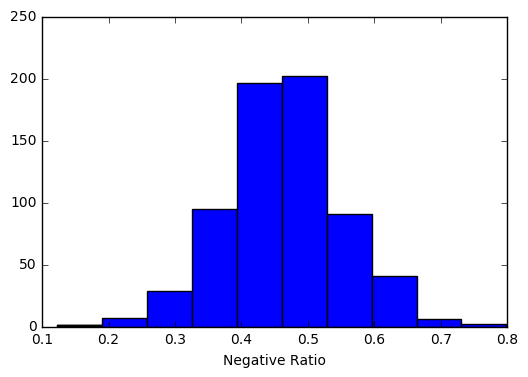
\includegraphics[scale=0.3]{neg_lm}$\quad$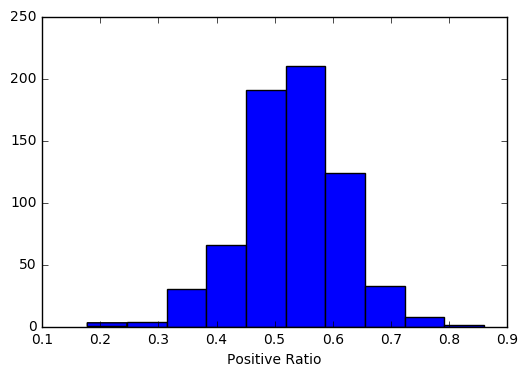
\includegraphics[scale=0.3]{pos_lm}$\quad$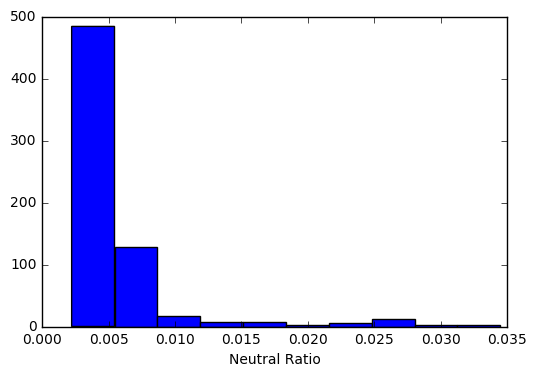
\includegraphics[scale=0.3]{neutral_lm}
\end{quotation}
\begin{center}
Figure7: LM Sentiment Histogram
\par\end{center}
\begin{quotation}
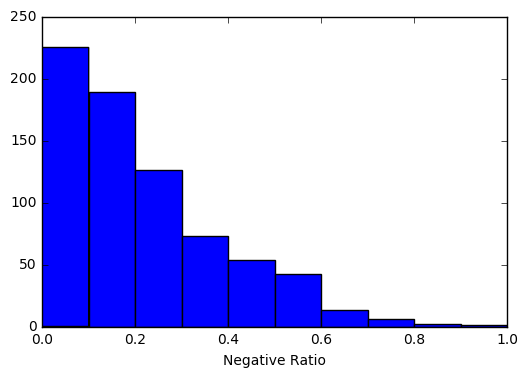
\includegraphics[scale=0.3]{neg_stock}$\quad$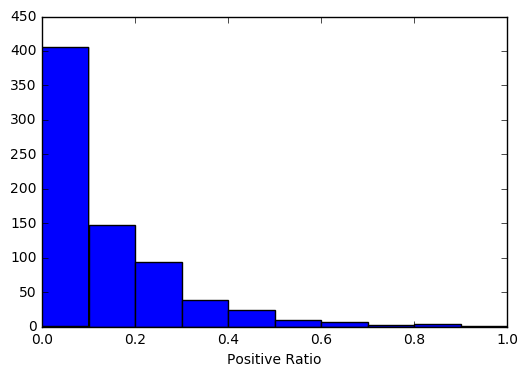
\includegraphics[scale=0.3]{pos_stock}$\quad$\includegraphics[scale=0.3]{neutral_stock}
\end{quotation}
\begin{center}
Figure 8: OF Sentiment Histogram 
\par\end{center}
$\quad\;$From the histogram, we could see that LM give more sentimental
judgement than OF. This might cause by LM is a financial dictionary,
which give more accurate sentiment judgement in our news dataset.
So in the following prediction, we use LM ratio as our sentiment factor,
which is number of negative words divided by number of positive words.

Then we visualize our sentiment factor time-series plot with DJIA
daily return to see the pattern.
\begin{center}
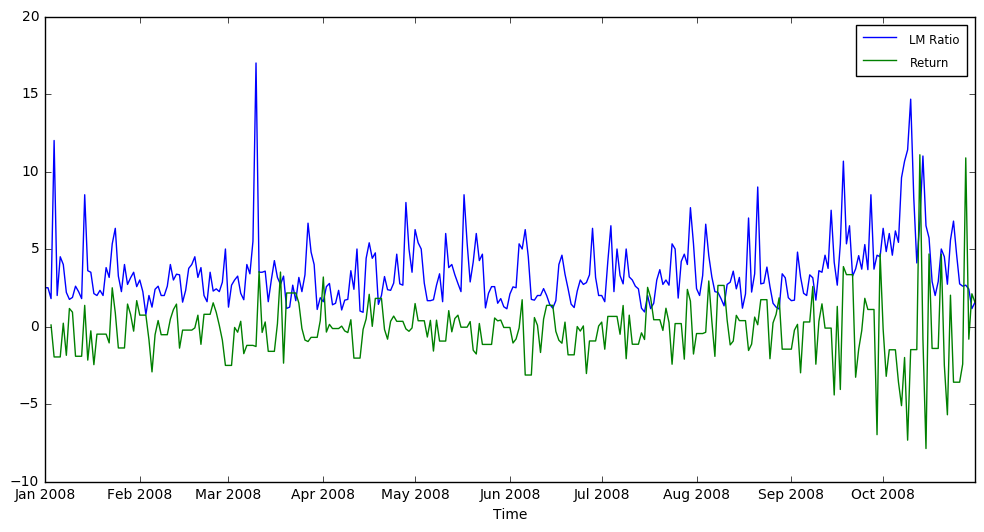
\includegraphics[scale=0.4]{new_finance}
\par\end{center}
\begin{center}
Figure 10: LM ratio and DJIA returns time-series 
\par\end{center}
$\;\quad$From this graph, we could clearly see that if our LM ratio
increase, which means the stock market sentiment is bearish, we could
see the following DJIA return will decrease and be negative. On the
other hand, if our LM ratio decrease, indicating the stock market
becomes bullish, the following DJIA return will increase and be positive.
And we should notice the lag is reasonably small in time, basically
around 5 days. 

So we use 5-day and 10-day lagged LM ratio to predict the up and down
of DJIA by using 30-days floating windows. We fit four different models:
logistic loss, SVM, Latent Dirichlet Allocation(LDA) and Quadratic
Discriminant Analysis(QDA) by using \emph{ScikitLearn} in Python.
The latter two models are popular neural network classification models.\\

\begin{center}
\includegraphics[scale=0.25]{logistic}$\quad$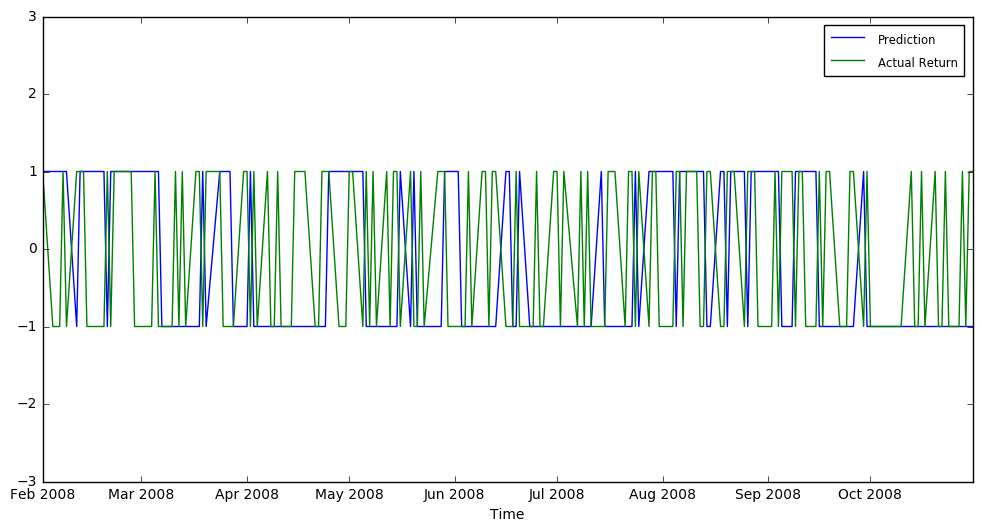
\includegraphics[scale=0.25]{svm}
\par\end{center}
\begin{flushleft}
$\qquad\;$Figure 11: Logistic regression prediction$\qquad\qquad$
Figure 12: SVM prediction
\par\end{flushleft}
$\;\quad$As we could see from the plots, the prediction results are
not as accurate. However, what we find interesting is that our predictor
seems like a smoother for the fluctuation of the stock market, which
means we predict the overall trend of market well but could not capture
daily fluctuation of stock market. 

Notice that here we use only lagged sentiment factors to predict the
stock index, which misses important information like the historical
performance of the index. Also, we find that using the whole finance
sector news as sentiment to predict the index trend is of difficulty
since we need to assign each news with accurate weight for its impact
on stock market. This is something we think makes our prediction not
as satisfatory. 

Therefore, in the next part, we narrow down our research to predict
single stock performance using sentiment factor. We set up a basis
prediction model using famous Fama-French 3 factor model, then we
add our sentiment factor to see if it improves the prediction accuracy.
\end{quotation}

\section{Single Stock Prediction }
\begin{quotation}
In this part, we focus on predicting single stock GE up and down by
using data from \emph{Quandl. }The dataset contains average sentiment
and impact scores computed on all articles related to GE, published
in last 24 hours. Article sentiment(AS) measures the average sentiment
of all the articles related to GE, taking values between -1 and 1.
Impact score(IS) gives us the average predicted impact of articles
on the stock price of GE, taking values between 0 and 100. 

We choose the Fama-French 3 factor model as our basis model. 
\[
r=R_{f}+\beta_{1}(r_{m}-r_{f})+\beta_{2}SMB+\beta_{3}HML+\varepsilon
\]

Here $r_{m}$ stands for market portfolio return, and $r_{f}$ is
the risk-free return rate. $SMB$ stands for ``Small (market capitalization)
Minus Big'' and $HML$ for ``High (book-to-market ratio) Minus Low''.
They measure the historic excess return of small caps over big caps
and of value stocks over growth stocks. These factors are calculated
with combinations of portfolios composed by ranked stocks and available
historical data. Historical values are accessed on \emph{Kenneth French's
web page}. 

Adding our sentiment factor, our model is formulated as
\[
y_{t}=f\left(\left(\alpha_{i}(r_{m}-r_{f})_{t-i}\right)_{i=1}^{k},\left(SMB_{t-i}\right)_{i=1}^{k},\left(HML_{t-i}\right)_{i=1}^{k},IS_{i-m},AS_{i-m}\right)
\]

where $k$ stands for the lagged period of Fama-French factors, and
$m$ is the lagged period for impact score and article sentiment. 

For classifier $y$, we first try binary classification, that is,
$1$ for positive return and $-1$ for negative return. Then we reflect
that three-class may be a more reasonable choice since there are quiet
time in stock market. So in the multiclass classification setting,
\[
y_{t}=\begin{cases}
1 & r_{t}>c\\
0 & |r_{t}|\leq c\\
-1 & r_{t}<-c
\end{cases}
\]

where $c$ is the threshold value for distinguish fluctuation and
quiet time. $c=0$ is binary classification.

We use SVM to fitted this model, i.e solving coefficients $w$ by
\[
minimize\stackrel[i=1]{n}{\sum}l_{hinge}(x_{i},y_{i};w)+\lambda r(w)
\]

We use three types of kernel here: linear, polynomial and Gaussian
radial basis function. We use $l_{1}$ and $l_{2}$ as our regularizers
$r(w)$.

In addition, we try the multilayer perceptron (MLP), which is a modification
of the standard linear perceptron and can distinguish data that are
not linearly separable.

Specifically, we use expanding window for fitting the model in this
part to use as much information till now as possible. That is, we
use data up to the first test day as our training dataset.

For different threshold value $c$, we have the following results
(in correctness days):
\begin{itemize}
\item $c=0$
\end{itemize}
\end{quotation}
\begin{center}
\begin{tabular}{|c|c|c|c|c|c|}
\hline 
Test period & SVM (linear) & SVM (poly) & SVM (Gaussian) & MLP & Basis FF 3 factors (SVM poly)\tabularnewline
\hline 
\hline 
Aug 1 - 10 & 6 & 6 & 6 & 5 & 3\tabularnewline
\hline 
Aug 11 - 20 & 5 & 3 & 4 & 3 & 4\tabularnewline
\hline 
Aug 21 - 30 & 4 & 6 & 6 & 5 & 4\tabularnewline
\hline 
Sep 1- 10 & 7 & 7 & 6 & 5 & 5\tabularnewline
\hline 
Sep 11 - 20 & 4 & 6 & 3 & 6 & 3\tabularnewline
\hline 
Sep 21 - 30 & 8 & 8 & 9 & 6 & 5\tabularnewline
\hline 
Oct 1 - 10 & 6 & 3 & 5 & 3 & 5\tabularnewline
\hline 
Average & 5.714 & 5.571 & 5.571 & 4.71 & 4.14\tabularnewline
\hline 
\end{tabular}
\par\end{center}
\begin{itemize}
\item $c=0.1$
\end{itemize}
\begin{center}
\begin{tabular}{|c|c|c|c|c|c|}
\hline 
Test period & SVM (linear) & SVM (poly) & SVM (Gaussian) & MLP & Basis FF 3 factors (SVM poly)\tabularnewline
\hline 
\hline 
Aug 1 - 10 & 6 & 7 & 5 & 4 & 2\tabularnewline
\hline 
Aug 11 - 20 & 4 & 4 & 3 & 4 & 4\tabularnewline
\hline 
Aug 21 - 30 & 3 & 4 & 4 & 5 & 4\tabularnewline
\hline 
Sep 1- 10 & 7 & 9 & 7 & 2 & 5\tabularnewline
\hline 
Sep 11 - 20 & 5 & 5 & 7 & 6 & 4\tabularnewline
\hline 
Sep 21 - 30 & 7 & 6 & 7 & 6 & 5\tabularnewline
\hline 
Oct 1 - 10 & 6 & 3 & 5 & 4 & 4\tabularnewline
\hline 
Average & 5.428 & 5.285 & 5.857 & 4.43 & 4.00\tabularnewline
\hline 
\end{tabular}
\par\end{center}
\begin{quotation}
$\;\quad$In the above model, we use the past data to predict the
following 10 trading days GE stock's ups and downs. The overall correctness
of our prediction is around 58\%, which is quite reasonable since
we found in previous literature the best prediction is nearly 56\%.
Comparing to our basis Fama-French 3 factor model, our prediction
improve the accuracy of prediction by 37.9\%.

We find that MLP does not give us a good result may because that we
use nearly 200 trading days data as our training dataset, which might
be too small to fit a neural network model, so it might cause overfitting
problem. The SVM with linear kernel produce the best result in our
test set.

Finally, we construct a simple trading strategy based on our prediction.
Here we also use expanding window to fit the model. If we predit GE
will go up tomorrow, we long at the close price today. If we predit
GE will go down tomorrow, we short the GE at the close price today.
And if there are two consecutive rise or fall, we do not change position
at the end of today. We plot our cumulative profits as follows with
comparison with basis Fama-French 3 factor prediction model.\\

\begin{center}
\includegraphics{strategy}
\par\end{center}
$\;\quad$In this simple trading strategy, we find that adding sentiment
could greatly improve our cumulative profits in two-month trading
day, compared to the famous Fama-French 3 factor model. 
\end{quotation}

\section{Conclusion and Future Work}
\begin{quotation}
The goal of our research is to unearth the relationship between the
sentiment of stock market and its trend. 

In the first part, we generate our sentiment factor by web scraping
google news of the whole finance sector. Then we tested the Granger
causality to prove there is predictability of our sentiment factor
to stock index prices. Then we use logistic loss, SVM, Latent Dirichlet
Allocation(LDA) and Quadratic Discriminant Analysis(QDA) to build
up four classfication models by 30-days rolling windows. In these
model, the only explanatory variables are 5-days and 10-days lagged
sentiment factors. As a result, what we find interesting is that our
predictor seems like a smoother for the fluctuation of the stock market,
which means we predict the overall trend of market well but could
not capture daily fluctuation of stock market. So we conjecture that
there might be two reasons for the result being not as accurate. First,
we use too broad information as our sentiment training set, which
might includes redundant information. Also, we might need other explanatory
variables as our basis model and add sentiment to see if it improves
the prediction.

So in the second part of our research, we narrow down our research
to predict single stock performance using sentiment factor. We set
up a basis prediction model using famous Fama-French 3 factor model,
then we add our sentiment factor to see if it improves the prediction
accuracy. We train SVM and MLP (neural network model) model by expanding
windows. In the out-of-sample test, our prediction improve the accuracy
of prediction by 37.9\% comparing to our basis Fama-French 3 factor
model. 

Finally, we build up a simple trading strategy based on our prediction
results. We greatly improve the cumulative profits compared to Fama-French
3 factor model over the 60 days.

In the end, its worth mentioning that our analysis could extend in
many different ways. First, we could train more financial specific
classfier by assigning the keywords in our sentiment dictionary with
larger weights. Second, google news headers might not be map the real
financial investor sentiment exactly, we could consider expend our
text data scope to news content and financial blogs for a better sentiment
factor. Third, we might include more fluctuating period such as financial
crisis to test the robustness of our factor. All these remains as
area of future research.
\end{quotation}

\section{References}
\begin{quotation}
{[}1{]} J. Bollen and H. Mao. Twitter mood as a stock market predictor.
IEEE Computer, 44(10):91\textendash 94. 

{[}2{]} C.-C. Chang and C.-J. Lin. LIBSVM: A library for support vector
machines. ACM Transactions on Intelligent Systems and Technology,
2:27:1\textendash 27:27, 2011. 

{[}3{]} G. P. Gang Leng and T. M. McGinnity. An on-line algorithm
for creating self-organizing fuzzy neural networks. Neural Networks,
17(10):1477\textendash 1493. 

{[}4{]} A. Lapedes and R. Farber. Nonlinear signal processing using
neural network: Prediction and system modeling. In Los Alamos National
Lab Technical Report. 

{[}5{]} A. E. Stefano Baccianella and F. Sebastiani. Sentiwordnet
3.0: An enhanced lexical resource for sentiment analysis and opinion
mining. In LREC. LREC.
\end{quotation}

\end{document}
